%------------------
% General Settings
%------------------
\def \docTitle      {Data sheet}
\def \docSubTitle   {M102}
\def \productNumber {M102}
\def \productName   {Rotation Stage}
\def \docAuthor     {LK-Instruments}
\def \docRevision   {Rev. 001}
\def \docSubject    {\docAuthor \docTitle \docSubTitle}
\def \docKeywords   {\docAuthor, \productName, \productNumber, SMC2242, SMC4242}

\documentclass[a4paper, final, 12pt, oneside]{scrartcl}

%----------
% Packages
%----------
\usepackage{etex}
\reserveinserts{30}
\usepackage[utf8]{inputenc}
%\usepackage[latin1]{inputenc} % erlaubt Umlaute in der tex-Datei

\usepackage{slantsc}
\usepackage[urw-garamond]{mathdesign}
\usepackage{garamondx}
\usepackage[sfdefault]{sourcesanspro}    % SourceSan­sPro als serifenlose Schrift
\usepackage[T1]{fontenc}

\usepackage[english]{babel}              % For the hyphenations in different languages
\usepackage[intlimits]{amsmath}          % math symbols
\usepackage{braket}                      % Dirac braket notation
\usepackage{graphicx}                    % include pictures
\usepackage{color}
%\usepackage[shell]{gnuplottex}           % gnuplot in latex
\usepackage{pstricks}                    % post script tricks
\usepackage{listings}                    % enter programming code
\usepackage{fancyhdr}                    % make quite nice header/footer
%\usepackage[version=3]{mhchem}           % chemistry stuff
\usepackage{relsize}
\usepackage{afterpage}
\usepackage{gensymb}
\usepackage{textcomp}
\usepackage{multicol}
%\usepackage{subfig}
\usepackage{lipsum}
\usepackage{multirow,booktabs,colortbl,tabularx}
\usepackage{caption}
\usepackage{subcaption}


%\usepackage{pgfplots}
%\usepackage{tikz}                        % beautiful plots
%\pgfplotsset{compat = newest}
\usepackage{units}                       % easy to use number-unit-package
\usepackage[section]{placeins}           % Float barrier for sections.


\usepackage{listings}					% erlaubt Quellcode mit Zeilenumbruechen

%----------------
% PDF properties
%----------------
\usepackage[
  pdftitle={\docAuthor~\docSubTitle~\docTitle}
 ,pdfsubject={\docSubject}
 ,pdfauthor={\docAuthor}
 ,pdfkeywords={\docKeywords}
 ,pdfcreator={\docAuthor}
 ,pdfstartview=Fit                       % startseite ganz anzeigen
 ,pdfborder={0 0 0}                      % links ohne umrandungen
 ,pdfdisplaydoctitle=true                % pdftitle statt dateinamen anzeigen
 ,pdfcenterwindow=true                   % position pdf in center of the screen
 ,setpagesize=true
]{hyperref}

%-------------------
% Header und Footer
%-------------------
\fancyhf{}        % clear all header/footer
\renewcommand{\headrulewidth}{0pt}
%\renewcommand{\sectionmark}[1]{\markboth{#1}{}}
%\renewcommand{\subsectionmark}[1]{\markright{#1}}
\fancyhead[RE,RO]{\productNumber}
\fancyfoot[LE,LO]{\docAuthor}
\fancyfoot[CE,CO]{\docRevision}
\fancyfoot[RE,RO]{\thepage}

\pagestyle{fancy}

% number equations with sections before equation-index
\numberwithin{equation}{section}
\numberwithin{table}{section}
\numberwithin{figure}{section}

%---------------------
% My code definitions
%---------------------

\newtheorem{envdefinition}{Definition}[section]
\newtheorem{envsatz}{Satz}

% special numbers and letters
\renewcommand{\i}{\mathrm{i}}                  % complex i
\newcommand{\e}{\mathrm{e}}                    % Eulers number
\renewcommand{\phi}{\varphi}                   % nicer phi
\renewcommand{\epsilon}{\varepsilon}           % nicer epsilon
\renewcommand{\theta}{\vartheta}               % nicer theta
\renewcommand{\rho}{\varrho}                   % nicer rho
%\newcommand{\degree}{^{\circ}}                 % degree-circle

% vectors and matrices
\renewcommand{\vec}[1]{\boldsymbol{#1}}
\newcommand{\Vek}[3]{\left(\begin{array}{c}#1\\#2 
\ifthenelse{\equal{#3}{}}{}{\\#3}\end{array}\right)}

% integral and derivative stuff:
\renewcommand{\d}[1]{\;\mathrm{d}#1}           % integeration d
% total derivative
\newcommand{\td}[1]{\frac{\mathrm{d}}{\mathrm{d}#1}\,}
\newcommand{\pd}[1]{\partial_{#1}\,}             % partial derivative

% Braket notation
\renewcommand{\bra}{\Bra}
\renewcommand{\ket}{\Ket}
\renewcommand{\braket}{\Braket}
\renewcommand{\set}{\Set}

% plus-minus with braces
\newcommand{\PM}{\ensuremath{\substack{+\\[-0.25em]-}\,}}
\renewcommand{\pm}{\PM}
\newcommand{\pmp}{\ensuremath{\substack{\mathsmaller{(}+\mathsmaller{)}\\[-0.25em]-}\,}}
\newcommand{\pmm}{\ensuremath{\substack{+\\[-0.25em]\mathsmaller{(}-\mathsmaller{)}}\,}}

\setlength{\columnsep}{40.0pt}

%----------------------------------------------------------
% let the party start
%----------------------------------------------------------
\begin{document}
\setlength{\parindent}{0pt}

\thispagestyle{empty}

\begin{minipage}{\textwidth}
  \begin{minipage}[h]{0.11\textwidth}
      
\includegraphics[width=1\textwidth]{../general/logo_black.pdf}
  \end{minipage}
  \hfill
  \begin{minipage}[h]{0.7\textwidth}
      {\huge \textbf{\textsf{\productName}}} \hfill
      {\huge \textbf{\textsf{\productNumber}}}
  \end{minipage}
\end{minipage} 

\vspace*{5pt}
\rule{\textwidth}{0.4pt}

\begin{multicols}{2}
\subsection*{Features}
\begin{itemize}
  \item[] Hall-sensor controlled automatic zero-positioning
  \item[] Robust design
  \item[] Load on motor axis
\end{itemize}
\FloatBarrier

\subsection*{Applications}
\begin{itemize}
  \item[] Changing optical filters
  \item[] Neutral density filter positioning
\end{itemize}
\FloatBarrier

\subsection*{Description}
The LK-Instruments M102 is a robust rotation stage designed for either carrying optical elements or being used in custom applications. It can be mounted to the experimental setup in any orientation utilizing standard M6 screws, set screws, posts and post holders.
\end{multicols}
\noindent\rule{\textwidth}{0.4pt}
\vspace*{0.5cm}

\centerline{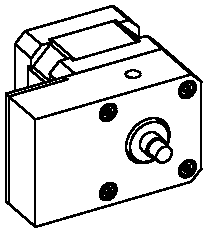
\includegraphics[width=0.5\textwidth]{./drawings/M102_iso.pdf}}

\vfill
\begin{minipage}{\textwidth}
  \begin{minipage}[t]{0.49\textwidth}
      
    
  \end{minipage}
  \hfill
  \begin{minipage}[t]{0.49\textwidth}
    \begin{flushright}
    {\footnotesize LK-Instruments\\
             Welzheimer Str. 49\\
             71554 Weissach im Tal\\
             Germany\\
             \href{http://www.lk-instruments.com}{www.lk-instruments.com}}
    \end{flushright}
  \end{minipage}
\end{minipage}






\FloatBarrier

\newpage
\subsection*{Specifications}
$T_A = \unit[25]{^{\circ}C}$ and 50\% RH unless otherwise noted.
\newcolumntype{C}[1]{>{\centering\arraybackslash}p{#1}}
\begin{table}[!htp]
  \centering
  \begin{tabular}{C{2.4cm} C{2cm} *{3}{C{1cm}} *{3}{C{1cm}} C{1.5cm} }
    \toprule
    \textbf{Parameter} & \textbf{Conditions} &
    \multicolumn{3}{p{3cm}}{\centering\textbf{M102A}} &
    \multicolumn{3}{p{3cm}}{\centering\textbf{M102B}} &
    \textbf{Unit} \\
    \cmidrule(lr){3-5} \cmidrule(lr){6-8}
    & &
    Min & Typ & Max &
    Min & Typ & Max &\\
    \toprule
    Current &  & 0.1 & 1.3 & 1.33 & 0.1 & 1.65 & 1.68 & A/Phase\\ \midrule
    Holding torque & Microst.=1, Curr.=Max & & 22 & & & 44 & & Ncm \\ \midrule
    Step angle & Microst.=1 & & 0.9 & & & 0.9 & & deg \\ \midrule
    Unidirectional repeatability &  & & 0.045 & & & 0.045 & & deg \\ \midrule
    Bidirectional repeatability &  & & 0.045 & & & 0.045 & & deg \\ \midrule
    Gear ratio &  & & 1 & & & 1 & &  \\ \midrule
    Velocity & Microst.=1, 2 ms/step & & 450 & & & 450 & & deg/s \\ \midrule
    Load capacity & radial/axial & &  & 20/7 & &  & 20/7 & N \\ \midrule
    Weight &  & & 0.38 & & & 0.51 & & kg \\ \midrule
    Temperature range &  & -10 &  & 50 & -10 &  & 50 & $^{\circ}$C \\
    \bottomrule
  \end{tabular}
\end{table}

\FloatBarrier
\newpage

\subsection*{Outer Dimensions}
All dimensions in millimeters.\\
With $A = \unit[33.5]{mm}$ for M102A and $A = \unit[47]{mm}$ for M102B.
\begin{figure}[!htp]
  \centering
  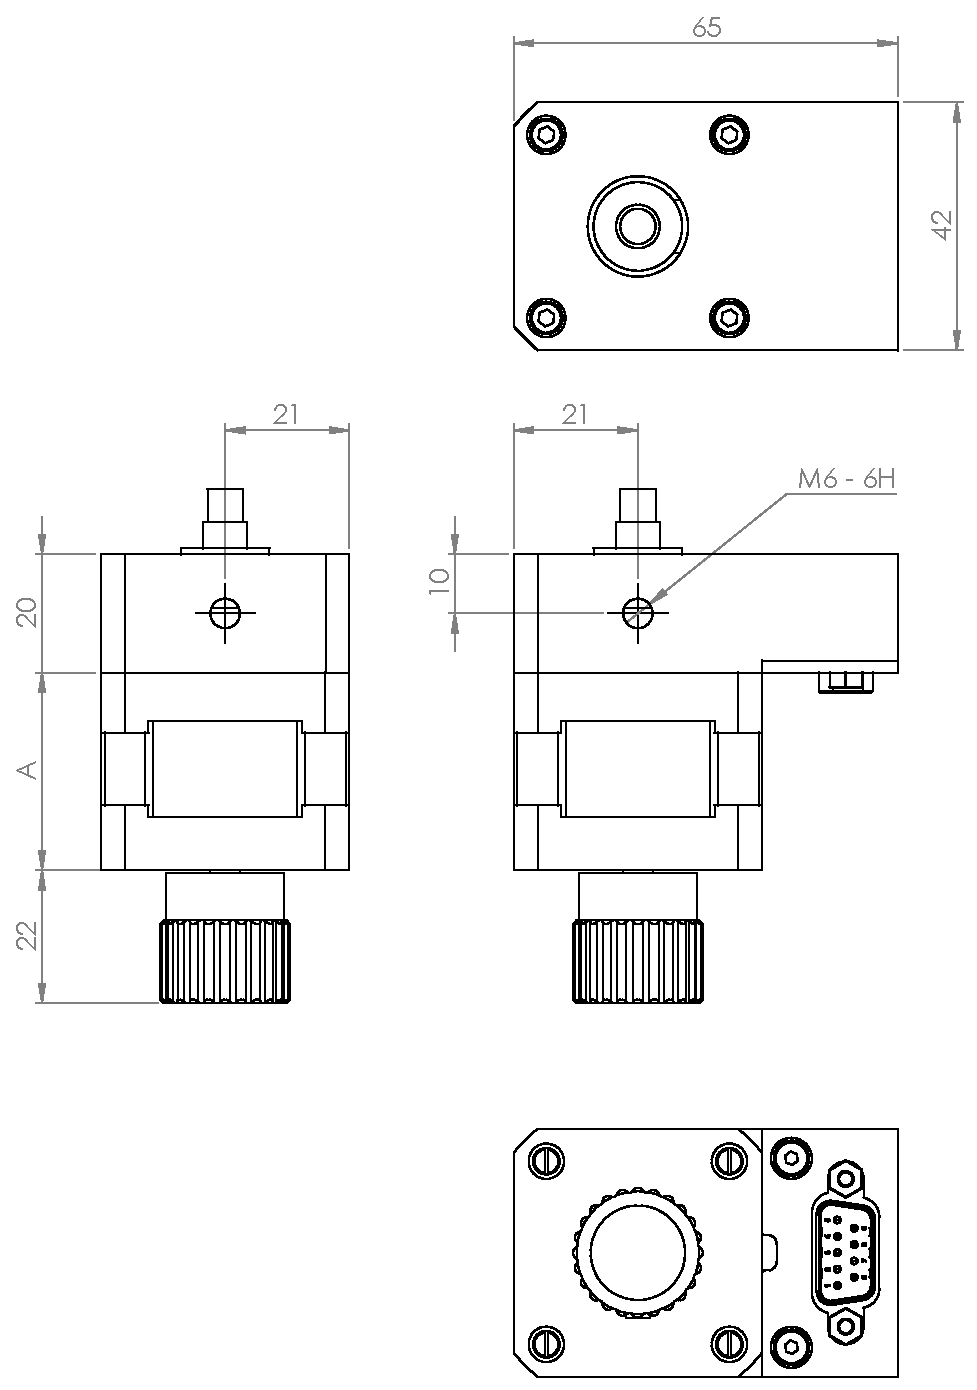
\includegraphics[angle=0,origin=c,width=0.8\textwidth]{./drawings/M102_outline_dimensions.pdf}
\end{figure}
%\vfill
\FloatBarrier

\subsection*{Pin Configuration}
\begin{minipage}{\textwidth}
  \begin{minipage}[b]{0.49\textwidth}
    \centering
    D-SUB-9 female connector\\
    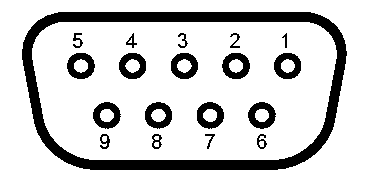
\includegraphics[width=0.6\textwidth]{./drawings/Numbered_DE9_female_Diagram.pdf}\\
    Front view
  \end{minipage}
  \hfill
  \begin{minipage}[b]{0.49\textwidth}
    \centering
    \begin{tabular}{cc}
      \toprule
      \textbf{Pin} & \textbf{Function} \\
      \toprule
      1 & Phase B1 \\ \midrule
      2 & Phase B2\\ \midrule
      3 & Phase A2 \\ \midrule
      4 & Phase A1 \\ \midrule
      5 & Ground \\ \midrule
      6 & +5V \\ \midrule
      7 & Zero sens \\ \midrule
      8 & NC \\ \midrule
      9 & NC \\ \midrule
      Shield & NC \\
      \bottomrule
    \end{tabular}
  \end{minipage}
\end{minipage}
\FloatBarrier

\subsection*{Ordering Information}
\begin{table}[!hp]
 % \centering
  %\begin{tabular}{C{2cm} C{3cm}}
  \begin{tabular}{ll}
    \toprule
    \textbf{Model} & \textbf{Description}\\
    \toprule
    M102A   & $\unit[22]{Ncm}$ holding torque, with rotary knob \\
    M102ANK & $\unit[22]{Ncm}$ holding torque, without rotary knob \\
    M102B   & $\unit[44]{Ncm}$ holding torque, with rotary knob \\
    M102BNK & $\unit[44]{Ncm}$ holding torque, without rotary knob \\
    \bottomrule
  \end{tabular}
\end{table}















\FloatBarrier
\vfill
\end{document}
